\documentclass{standalone}

\usepackage{hyperref}
\usepackage{tikz}

\usetikzlibrary{decorations.pathreplacing,
  arrows,
  calc,
  decorations.pathmorphing,
  decorations.pathreplacing,
  decorations.markings,
  positioning,
  shapes,
  3d
}

\tikzstyle{snakearrow} = [decorate, decoration={pre length=0.1cm,
  post length=0.1cm, snake, amplitude=.13mm,
  segment length=1mm},thick, ->]
\tikzstyle{densely rounded dotted} = [line cap=round, dash pattern=on 0pt off 1.3\pgflinewidth]

\ifpdf
  % Ensure reproducible output
  \pdfinfoomitdate=1
  \pdfsuppressptexinfo=-1
  \pdftrailerid{}
  \hypersetup{
    pdfcreator={},
    pdfproducer={}
  }
\fi

\def\statewidth{0.7}
\def\stategap{0.2}

\begin{document}
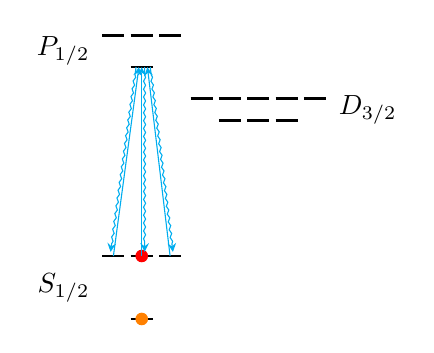
\begin{tikzpicture}[scale=0.4]
  % S 1/2
  \begin{scope}
    \draw[line width=1] ({\statewidth*-1.5-\stategap}, 0) -- coordinate (S1m1) ({\statewidth*-0.5-\stategap}, 0);
    \draw[line width=1] ({\statewidth*-0.5}, 0) -- coordinate (S10) ({\statewidth*0.5}, 0);
    \draw[line width=1] ({\statewidth*0.5+\stategap}, 0) -- coordinate (S11) ({\statewidth*1.5+\stategap}, 0);

    \node[left] at ({\statewidth*-1.5-\stategap-0.1}, -1) {$S_{1/2}$};

    \draw[line width=1] ({\statewidth*-0.5}, -2) -- coordinate (S00) ({\statewidth*0.5}, -2);
  \end{scope}

  % P 1/2
  \begin{scope}[shift={(0, 7)}]
    \draw[line width=1] ({\statewidth*-1.5-\stategap}, 0) -- coordinate (P1m1) ({\statewidth*-0.5-\stategap}, 0);
    \draw[line width=1] ({\statewidth*-0.5}, 0) -- coordinate (P10) ({\statewidth*0.5}, 0);
    \draw[line width=1] ({\statewidth*0.5+\stategap}, 0) -- coordinate (P11) ({\statewidth*1.5+\stategap}, 0);

    \node[left] at ({\statewidth*-1.5-\stategap-0.1}, -0.5) {$P_{1/2}$};

    \draw[line width=1] ({\statewidth*-0.5}, -1) -- coordinate (P00) ({\statewidth*0.5}, -1);
  \end{scope}

  % D 3/2
  \begin{scope}[shift={(3.7, 5)}]
    \draw[line width=1] ({\statewidth*-2.5-\stategap*2}, 0) -- coordinate (D2m2) ({\statewidth*-1.5-\stategap*2}, 0);
    \draw[line width=1] ({\statewidth*-1.5-\stategap}, 0) -- coordinate (D2m1) ({\statewidth*-0.5-\stategap}, 0);
    \draw[line width=1] ({\statewidth*-0.5}, 0) -- coordinate (D20) ({\statewidth*0.5}, 0);
    \draw[line width=1] ({\statewidth*0.5+\stategap}, 0) -- coordinate (D21) ({\statewidth*1.5+\stategap}, 0);
    \draw[line width=1] ({\statewidth*1.5+\stategap*2}, 0) -- coordinate (D22) ({\statewidth*2.5+\stategap*2}, 0);

    \node[right] at ({\statewidth*2.5+\stategap*2+0.1}, -0.35) {$D_{3/2}$};

    \draw[line width=1] ({\statewidth*-1.5-\stategap}, -0.7) -- coordinate (D1m1) ({\statewidth*-0.5-\stategap}, -0.7);
    \draw[line width=1] ({\statewidth*-0.5}, -0.7) -- coordinate (D10) ({\statewidth*0.5}, -0.7);
    \draw[line width=1] ({\statewidth*0.5+\stategap}, -0.7) -- coordinate (D11) ({\statewidth*1.5+\stategap}, -0.7);
  \end{scope}

  \fill[orange] (S00) circle (0.2);
  \fill[red] (S10) circle (0.2);
  \draw[->, >=stealth, cyan, line width=0.4] (S10) -- (P00);
  \draw[->, >=stealth, cyan, line width=0.4] (S1m1) -- ($(P00) + (-0.09, 0)$);
  \draw[->, >=stealth, cyan, line width=0.4] (S11) -- ($(P00) + (0.18, 0)$);

  \draw[->, >=stealth, snakearrow, cyan, line width=0.4] ($(P00) + (-0.18, 0)$) -- ($(S1m1) + (-0.09, 0.13)$);
  \draw[->, >=stealth, snakearrow, cyan, line width=0.4] ($(P00) + (0.09, 0)$) -- ($(S10) + (0.09, 0.13)$);
  \draw[->, >=stealth, snakearrow, cyan, line width=0.4] ($(P00) + (0.27, 0)$) -- ($(S11) + (0.09, 0.13)$);
\end{tikzpicture}
\end{document}
